\documentclass[]{article}

% Imported Packages
%------------------------------------------------------------------------------
\usepackage{amssymb}
\usepackage{amstext}
\usepackage{amsthm}
\usepackage{amsmath}
\usepackage{enumerate}
\usepackage{fancyhdr}
\usepackage[margin=1in]{geometry}
\usepackage{graphicx}
%\usepackage{extarrows}
%\usepackage{setspace}
%\usepackage{xcolor}
\usepackage{color}
\usepackage[hyphens]{url}
\usepackage{hyperref}
%------------------------------------------------------------------------------

% Header and Footer
%------------------------------------------------------------------------------
\pagestyle{plain}  
\renewcommand\headrulewidth{0.4pt}                                      
\renewcommand\footrulewidth{0.4pt}                                    
%------------------------------------------------------------------------------

% Title Details
%------------------------------------------------------------------------------
\title{Deliverable \#1 Template : Software Requirement Specification (SRS)}
\author{SE 3A04: Software Design II -- Large System Design}
\date{}
                            
%------------------------------------------------------------------------------

% Document
%------------------------------------------------------------------------------
\begin{document}

\maketitle	
\noindent{\bf Tutorial Number:} T0x\\
{\bf Group Number:} Gx \\
{\bf Group Members:} 
\begin{itemize}
	\item Group Member Name (as listed in Avenue)
	\item You do not need to use student \#s or macid (keep those private).
\end{itemize}

\section*{IMPORTANT NOTES}
\begin{itemize}
	\item Be sure to include all sections of the template in your document regardless whether you have something to write for each or not
	\begin{itemize}
		\item If you do not have anything to write in a section, indicate this by the \emph{N/A}, \emph{void}, \emph{none}, etc.
	\end{itemize}
	\item Uniquely number each of your requirements for easy identification and cross-referencing
	\item Highlight terms that are defined in Section~1.3 (\textbf{Definitions, Acronyms, and Abbreviations}) with \textbf{bold}, \emph{italic} or \underline{underline}
	\item For Deliverable 1, please highlight, in some fashion, all (you may have more than one) creative and innovative features. Your creative and innovative features will generally be described in Section~2.2 (\textbf{Product Functions}), but it will depend on the type of creative or innovative features you are including.
\end{itemize}

\newpage
\section{Introduction}
\label{sec:introduction}
% Begin Section

\begin{itemize}
	\item Provide an overview of the document/SRS.
\end{itemize}


\subsection{Purpose}
\label{sub:purpose}
% Begin SubSection
This SRS outlines the functional and non-functional requirements for the DealCheck app, detailing the system's design, features, and use cases. The intended audience includes internal stakeholders of DealCheck, such as project managers, software developers, product designers, marketing, customer support, executives, and investors. The document is written to be easily understood by all involved parties, with no prior technical expertise required.
% End SubSection

\subsection{Scope}
\label{sub:scope}

DealCheck is a mobile application that will allow users to request from the system a check on a car deal by providing any necessary data (car year, make, model, mileage, listing price, etc) and optional data (images, text description, etc.), which provides them with a rating of the car deal.
\hfill
\break

\noindent{Users are required to register an account on DealCheck to get access to all the features of the mobile application system. The users can make requests by filling out a “form” that captures all the data of a certain car to measure the fairness of the deal through the integrated experts. Furthermore, users can request recommendations for a car through the system by providing a description of their preferences (looks, engine, etc.) and requirements (price range, fuel efficiency, etc) for their car.}
\hfill
\break

\noindent{An objective of the system is to provide users with an easy and reliable way to get accurate estimates on the fairness of a car deal. Many people across the world are looking to buy a car, but are not very knowledgeable in the field. The DealCheck system acts as a guiding hand throughout the process of the user's search for their “perfect” car.}

%	\item Be consistent with similar statements in higher-level specifications (e.g., the system requirements specification), if they exist
% End SubSection

\subsection{Definitions, Acronyms, and Abbreviations}
\label{sub:definitions_acronyms_and_abbreviations}
% Begin SubSection
\begin{itemize}
\item \textbf{DealCheck:} The name of the mobile application being proposed.
\item \textbf{API:} Application Programming Interface, used to retrieve pricing data from external sources.
\item \textbf{AI:} Artificial Intelligence, for analyzing images and/or text input.
\item \textbf{SRS:} Software Requirements Specification document 
\item \textbf{Account Management Database:} A supporting entity that stores user login information and car valuation reports. 
\item \textbf{OS:} Operating System.
\item \textbf{Expert:} A software component that will process the data and provide a result to whether it thinks the car deal is good or not based on the experts algorithm.
\end{itemize}
% End SubSection

\subsection{References}
\label{sub:references}
\begin{enumerate}
    \item [\textbf{[1]}] W. L. in R.-B. U. Experience, “Best Font for Online Reading: No Single Answer,” Nielsen Norman Group, Apr. 24, 2022. Available at: \url{https://www.nngroup.com/articles/best-font-for-online-reading/}.
    
    \item [\textbf{[2]}] satyendra, “The Top 5 Web Scraping Challenges: Best Practices and Solutions,” Rayobyte, Aug. 03, 2023. Available at: \url{https://rayobyte.com/blog/web-scraping-solutions/} (accessed Feb. 02, 2025).
    
    \item [\textbf{[3]}] R. Lai, “The SOLID Principles: Writing Scalable \& Maintainable Code,” Medium, Jun. 28, 2023. Available at: \url{https://forreya.medium.com/the-solid-principles-writing-scalable-maintainable-code-13040ada3bca} (accessed Feb. 02, 2025).
\end{enumerate}

\subsection{Overview}
\label{sub:overview}
% Begin SubSection
Section 2 discusses the overall product description focusing on the product perspective, product functions,user characteristics, assumptions and dependencies, and apportioning of requirements. Section 3 contains the use case diagram illustrating the scenario of a user requesting a deal check on a car. Section 4 highlights the functional requirements, main business events and viewpoints. Section 5 provides the non-functional requirements talking about look and feel requirements, usability and humanity requirements, performance requirements, operational and environmental requirements, maintainability and support requirements, security requirements, cultural and political requirements and legal requirements. Section 6 holds the division of labour. Lastly, Section 7 discusses the innovative design feature.
% End SubSection

% End Section

\section{Overall Product Description}
\label{sec:overall_description}
% Begin Section

\begin{itemize}
	\item This section should describe the general factors that affect the product and its requirements. 
	\item It does not state specific requirements.
	\item It provides a \emph{background} for those requirements and makes them easier to understand.
\end{itemize}


\subsection{Product Perspective}
\label{sub:product_perspective}
% Begin SubSection
\begin{itemize}
	\item Put the product into perspective with other related products, i.e., context
	\item If the product is independent and totally self-contained, it should be stated here
	\item If the SRS defines a product that is a component of a larger system, then this subsection should relate the requirements of that larger system to the functionality of the software being developed. Identify interfaces between that larger system and the software to be developed.
	\item A block diagram showing the major components of the larger system, interconnections, and external interfaces can be helpful
\end{itemize}
% End SubSection

\subsection{Product Functions}
\label{sub:product_functions}
% Begin SubSection
\begin{itemize}
	\item Provide a \emph{summary} of the major functions that the software will perform.
	\begin{itemize}
		\item \textbf{Example}: An SRS for an accounting program may use this part to address customer account maintenance, customer statement, and invoice preparation without mentioning the vast amount of detail that each of those functions requires.
	\end{itemize}
	\item Functions should be organized in a way that makes the list of functions understandable to the customer or to anyone else reading the document for the first time 
	\item Present the functions in a list format - each item should be one function, with a brief description of it
	\item Textual or graphical methods can be used to show the different functions and their relationships
	\begin{itemize}
		\item Such a diagram is not intended to show a design of a product, but simply shows the logical relationships among variables
	\end{itemize} 
\end{itemize}
% End SubSection

\subsection{User Characteristics}
\label{sub:user_characteristics}
% Begin SubSection
	The DealCheck app is designed to be accessible and user-friendly for a wide range of users. It has the following expected qualifications for its users:
\begin{itemize}
    \item \textbf{Education Level:} Basic Literacy Skills\\
    Users with basic literacy skills in reading and writing should have no trouble navigating and using the app to evaluate car prices and request deal checks.
    
    \item \textbf{Technical Expertise:} Basic Knowledge of Smartphone Usage\\
    Users who are familiar with basic smartphone functions (such as navigating through apps, selecting options, and inputting text and images) should be able to easily use the app without requiring specialized technical knowledge.
    
    \item \textbf{Age Group:} 18+\\
    The app is aimed at adult users who are interested in buying or selling cars, meaning users are expected to be 18 years old or older. The interface is designed to be simple enough for all adult users to access and understand.
\end{itemize}
% End SubSection

\subsection{Constraints}
\label{sub:constraints}
% Begin SubSection
\begin{itemize}
    \item \textbf{Data Privacy Constraint}: The app must comply with local data protection laws such as GDPR or PIPEDA.
    \item \textbf{Project Timeline}: The amount of time allocated for the project will influence the number of additional features that can be implemented. It also impacts the overall development schedule and the resources available for the project.
    \item \textbf{Target Audience Constraint}: The system must be designed to cater to both novice and experienced car buyers.
    \item \textbf{Time Limit for Car Deal Valuation}: The system must provide the final valuation result (e.g., "Good Deal," "Bad Deal") within 5 seconds of receiving input.
\end{itemize}
% End SubSection

\subsection{Assumptions and Dependencies}
\label{sub:assumptions_and_dependencies}
% Begin SubSection
\begin{enumerate}
\item Assume that when a user posts a request for a deal check that all required input is provided before being processed
\item Innovative Feature: Users can request a car recommendation based on a provided description and set of requirements.
\item Assume data provided by the user is accurate.
\item The app requires an internet connection.
\item Assume the features of the app are only accessed by authenticated users.
\item Assume data from external sources is reliable and up-to-date.
\item Assume external APIs are available and reliable.
\item This app will only be used within Canada
\end{itemize}

Other assumptions that if changed, requirements may need to be updated:
\begin{enumerate}
\item The app shall work on the latest release of the Android OS.
\item Assume users of the system are looking to evaluate a car deal and not misuse the system.
\end{enumerate}
% End SubSection

\subsection{Apportioning of Requirements}
\label{sub:apportioning_of_requirements}
% Begin SubSection
\begin{itemize}
	\item Identify requirements that may be delayed until future versions of the system
\end{itemize}
% End SubSection

% End Section
\newpage
\section{Use Case Diagram}
\label{sec:use_case_diagram}
% Begin Section
\begin{figure}[h]
	\centering
	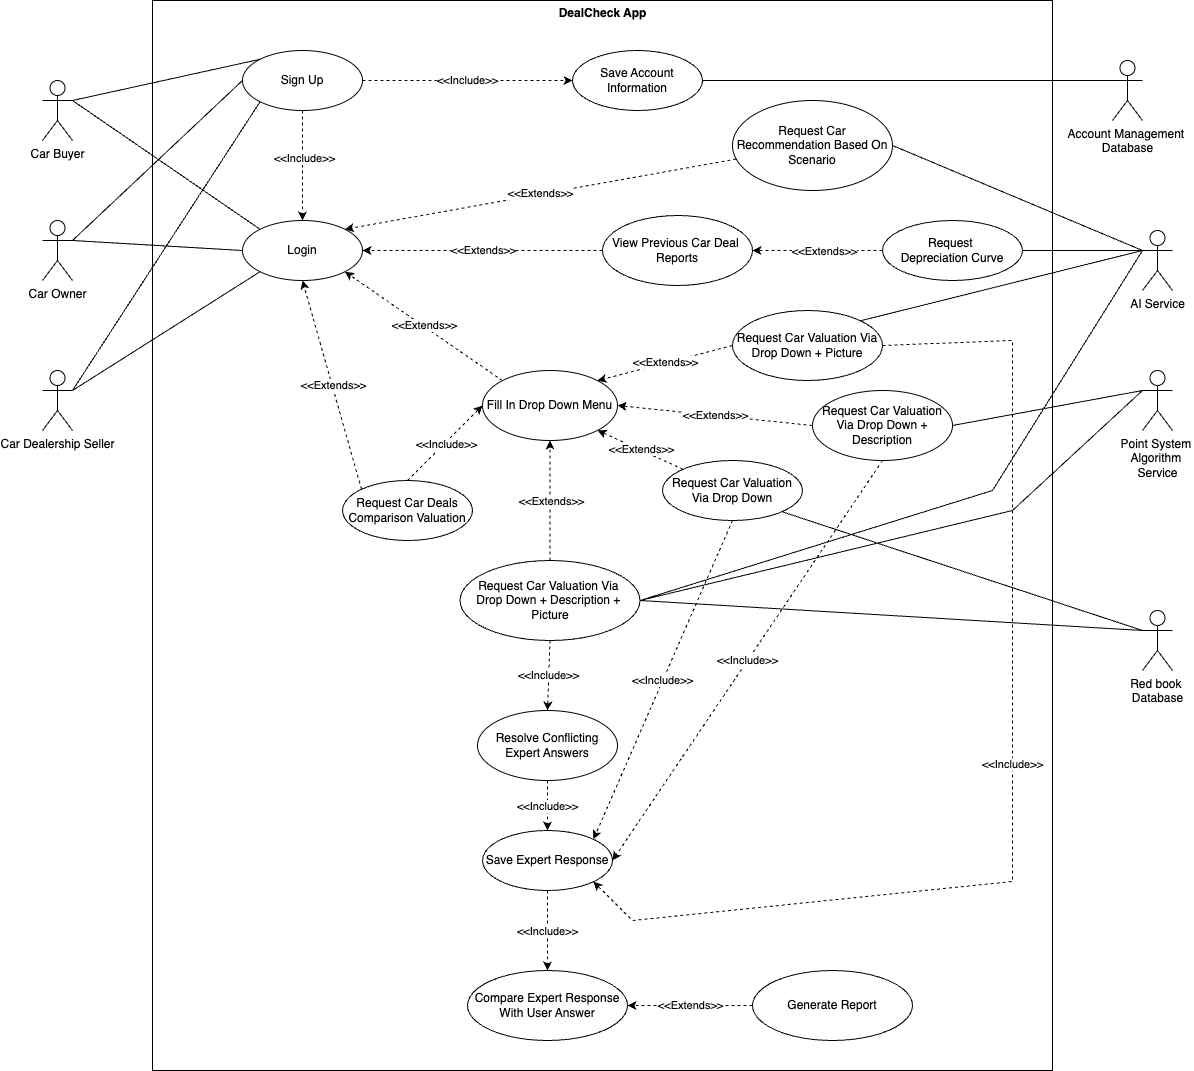
\includegraphics[scale=0.4]{Images/UseCase.png}
	\textbf{\caption{Use Case Diagram}}
	\label{fig:example}
\end{figure}
%In this section, select the most important Business Event that your system responds to and give its use case diagram.  Only one use case diagram is needed.  Give a brief textual description of the use case without repeating what is in the scenarios of the corresponding Business Event.

%
%
%
%This section should provide a use case diagram for your application. 
%\begin{enumerate}[a)]
%	\item Each use case appearing in the diagram should be accompanied by a text description. 
%\end{enumerate}
%% End Section

\section{Highlights of Functional Requirements}
\label{sec:functional_requirements}
% Begin Section
\begin{itemize}
	\item Specify all use cases (or other scenarios triggered by other events), organized by Business Event. 
	\item For each Business Event, show the scenario from every Viewpoint. You should have the same set of Viewpoints across all Business Events. If a Viewpoint doesn't participate, write N/A so we know you considered it still. You can choose how to present this - keep in mind it should be easy to follow. 
	\item At the end, combine them all into a Global Scenario.
	%\item Specify the "use cases" (or other triggering events) organized by Business Event. (The Global Scenario is what you might think of as a use case). Be sure to consider Business Events that aren't just triggered by users with goals (e.g. something happens in the environment that your system needs to respond to)
	\item Your focus should be on what the system needs to do, not how to do it. Specify it in enough detail that it clearly specifies what needs to be accomplished, but not so detailed that you start programming or making design decisions.
	\item Keep the length of each use case (Global Scenario) manageable. If it's getting too long, split into sub-cases.
	\item You are \emph{not} specifying a complete and consistent set of functional requirements here. (i.e. you are providing them in the form of use cases/global scenarios, not a refined list). For the purpose of this project, you do not need to reduce them to a list; the global scenarios format is all you need.
	\item Red text below is just to highlight where you need to insert a scenario - don't actually write it all in red.
\end{itemize}

\noindent {\bf Main Business Events:} \\

\noindent The business events considered include:

\begin{itemize}
	\item BE1 Request a deal valuation based on drop down menu input
	\item BE2 Request a deal valuation based on image and required text input
	\item BE3 Request a deal valuation with text description
	\item BE4 Request a depreciation curve for a previous car deal report
	\item BE5 Request a deal valuation based on text, drop down, and image input
	\item BE6 Request a car recommendation based on text information provided
	\item BE7 Request comparison between two or more car deals
	\item BE8 Account creation
	\item BE9 Account login
\end{itemize}

\noindent {\bf Viewpoints:} \\

\noindent The viewpoints considered include:

\begin{itemize}
	\item VP1 Users
	\item VP2 Customer Support (DealCheck)
	\item VP3 Marketing (DealCheck)
	\item VP4 Car Manufacturers
	\item VP5 Car Dealerships
\end{itemize}

\noindent {\bf Interpretation:} Specify any liberties you took in interpreting business events, if necessary. \\

\begin{enumerate}[{\bf {BE}1.}]

    \item User requests deal valuation based on drop-down menu \\    
	\textbf{Precondition:} User does not have an ongoing request within the system. The user must also be logged into their account on the app. The user must also know the basic information about their car (make, model, year, location).
    \begin{enumerate}[{\bf VP1.}]
      \item User \#1
        \textbf{Main Success Scenario}
        \begin{enumerate}[1.]
          \item User opens the DealCheck application.
          \item User selects “Check New Vehicle”.
          \item User enters relevant drop-down information (make, model, year, location).
          \item User enters their own guess for the deal in the guess check text box.
          \item User presses the ‘Submit’ button.
          \item System consults with the points-based algorithm.
          \item System compiles results from the algorithm.
          \item System returns results to the user and lets the user know if they were right or not.
          \item User saves the query by pressing ‘Save information’.
        \end{enumerate}
        \textbf{Secondary Scenario}
        \begin{enumerate}
          \item[4i.] User does not fill out drop-down inputs.
          \begin{enumerate}
            \item[4i.1] User neglects to fill out all drop-down inputs.
            \item[4i.2] Query failed.
          \end{enumerate}
        \end{enumerate}
      \item Customer Support (DealCheck) \#2
        \begin{enumerate}
          \item[6i.] System should provide an error page to indicate loss of internet connection and recommend trying again.
          \item[7ii.] System should provide users with guidelines for proper drop-down submission.
        \end{enumerate}
      \item Marketing (DealCheck) \#3
        \begin{enumerate}
          \item[9i.] System should provide suggestions of similar vehicles that have historically better prices.
        \end{enumerate}
      \item Car Manufacturers \#4 - N/A.
      \item Car Dealerships Staff \#5 - N/A.
    \end{enumerate}
    
    \textbf{Global Scenario:} \\
    \textbf{Precondition:} User does not have an ongoing request within the system. The user must also be logged into their account on the app. The user must also know the basic information about their car (make, model, year, location).
    \begin{enumerate}[{\bf 1.}]
      \item User opens the DealCheck application.
      \item User selects “Check New Vehicle”.
      \item User enters relevant drop-down information (make, model, year, location).
      \item User enters their own guess for the deal in the guess check text box.
      \item User presses the ‘Submit’ button.
      \item System consults with the points-based algorithm.
      \item System compiles results from the algorithm.
      \item System returns results to the user and lets the user know if they were right or not.
      \item User saves the query by pressing ‘Save information’.
    \end{enumerate}
    \textbf{Secondary Scenario}
    \begin{enumerate}
      \item[5i.] System loses internet connection upon form submission.
      \begin{enumerate}
        \item[5i.1] System is unable to perform the request.
        \item[5i.2] System fails.
      \end{enumerate}
      \item[4i.] User does not fill out drop-down inputs.
      \begin{enumerate}
        \item[4i.1] User neglects to fill out all drop-down inputs.
        \item[4i.2] Query failed.
        \item[4i.3] System should provide users with guidelines for proper drop-down submission.
      \end{enumerate}
    \end{enumerate}


	\item Business Event Name \#2
	\begin{enumerate}[{\bf VP1.}]
		\item Viewpoint Name \#1 \\
		\textcolor{red}{Insert Scenario Here}
		\item Viewpoint Name \#2 \\
		\textcolor{red}{Insert Scenario Here}
	\end{enumerate}
	{\bf Global Scenario:}\\
	\textcolor{red}{Insert Scenario Here}

\item Request a deal valuation with text description \#3 \\
    {\bf Precondition:} User does not have an ongoing request within the system. User is authenticated and logged into their account (as described in BE9).
    \begin{enumerate}[{\bf VP1.}]
        \item User \#1 \\
        {\bf Main Success Scenario}
        \begin{enumerate}[1.]
            \item User opens the DealCheck application.
            \item User selects to start a new deal check request.
            \item System requests user to enter mandatory fields.
            \begin{itemize}
                \item Car Price.
                \item Car model year.
                \item Car make.
                \item Car model.
                \item Car Mileage.
                \item Users' opinion on whether they think this deal is a good or bad deal.
            \end{itemize}
            \item System requests user to enter optional fields:
            \begin{itemize}
                \item Text Description.
            \end{itemize}
            \item User inserts mandatory and optional fields.
            \item User submits request.
            \item System provides submitted data to experts.
            \item System aggregates and displays report of expert results.
        \end{enumerate}
        
        {\bf Secondary Scenario} \\
		\begin{description}
			\item [6i.] User does not provide all mandatory fields:
			\begin{description}
				\item [6i.1] The system does not allow the user to submit the request until all mandatory fields have been provided.
			\end{description}
		
			\item [6ii.] System loses internet connection upon form submission.
			\begin{description}
				\item [6ii.1] System is unable to perform the request.
				\item [6ii.2] System displays an error message.
			\end{description}
		
			\item [6iii.] User provides an insufficient textual description.
			\begin{description}
				\item [6iii.1] System does not attempt to analyze the text or generate insights.
				\item [6iii.2] System notifies the user that the input is insufficient and prompts for additional details.
			\end{description}
		\end{description}
    
        \item Customer Support (DealCheck) \#2 \\
            \textbf{7i.} System should notify users when expert analysis is unavailable and recommend retrying later.
        \item Marketing (DealCheck) \#3 \\
            \textbf{9i.} System should suggest similar vehicles with better historical prices.
        \item Car Manufacturers \#4 \\
            NA
        \item Car dealership staff \#5 \\
            NA
    \end{enumerate}
    {\bf Global Scenario:}\\
    {\bf Precondition:} User does not have an ongoing request within the system. User is authenticated and logged into their account (as described in BE9).
    
    {\bf Main Success Scenario}
        \begin{enumerate}[1.]
            \item User opens the DealCheck application.
            \item User selects to start a new deal check request.
            \item System requests user to enter mandatory fields.
            \begin{itemize}
                \item Car Price.
                \item Car model year.
                \item Car make.
                \item Car model.
                \item Car Mileage.
                \item Users' opinion on whether they think this deal is a good or bad deal.
            \end{itemize}
            \item System requests user to enter optional fields:
            \begin{itemize}
                \item Text Description.
            \end{itemize}
            \item User inserts mandatory and optional fields.
            \item User submits request.
            \item System provides submitted data to experts.
            \item System aggregates and displays report of expert results.
        \end{enumerate}
        
        {\bf Secondary Scenario} \\
        \begin{description}
			\item [6i.] User does not provide all mandatory fields:
			\begin{description}
				\item [6i.1] The system does not allow the user to submit the request until all mandatory fields have been provided.
			\end{description}
		
			\item [6ii.] System loses internet connection upon form submission.
			\begin{description}
				\item [6ii.1] System is unable to perform the request.
				\item [6ii.2] System displays an error message.
			\end{description}
		
			\item [6iii.] User provides an insufficient textual description.
			\begin{description}
				\item [6iii.1] System does not attempt to analyze the text or generate insights.
				\item [6iii.2] System notifies the user that the input is insufficient and prompts for additional details.
			\end{description}

			\item [7i.] System should notify users when expert analysis is unavailable and recommend retrying later.

        	\item [9i.] System should suggest similar vehicles with better historical prices.
		\end{description}

\item User Requests Depreciation Curve for a Previous Car Deal Report \#4

{\bf Precondition:} User doesn't have an ongoing request within the system. Furthermore, the user has previously requested and saved a car deal report, and the system 
	has access to relevant data sources to determine the depreciation data.
	\begin{enumerate}[{\bf VP1.}]
		\item User \#1 \\
		{\bf Main Success Scenario}
		\begin{enumerate}[1.]
			\item User opens the DealCheck application.
			\item System requires the user to log in and displays the log-in fields.
			\item User enters login details.
			\item System successfully authenticates the user and showcases the homepage of DealCheck.
			\item User navigates to "Saved Reports."
			\item System showcases the previous car deal report.
			\item User selects a previous car deal report.
			\item System displays the car deal details along with an option to request a depreciation curve.
			\item User selects "View Depreciation Curve."
			\item System retrieves historical depreciation data for the selected car (make, model, year).
			\item System processes the depreciation curve using the AI service.
			\item System generates a depreciation curve based on past market trends and future projections.
			\item System displays the depreciation curve to the user, showing estimated price drops over time.
			\item System prompts the user with an option to save the depreciation curve for future reference.
			\item User selects to save the depreciation curve.
		\end{enumerate}
	\end{enumerate}
		{\bf Secondary Scenario}
		\begin{description}
			\item[6i.] User has no saved car deal reports.
			\begin{description}
				\item[6i.1] System notifies the user that no previous reports exist.
				\item[6i.2] System suggests checking recent car valuation requests or starting a new one.
			\end{description}
			
			\item[7i.] User selects the wrong car deal report.
			\begin{description}
				\item[7i.1] System allows the user to go back and select the correct report.
				\item[7i.2] System suggests filtering or searching reports by date, car model, or price.
			\end{description}
			
			\item[9i.] User wants depreciation data for a different region or country.
			\begin{description}
				\item[9i.1] System detects location settings and warns if data is unavailable for the selected region.
				\item[9i.2] System provides alternative data based on the closest available market.
			\end{description}
		\end{description}  
		
		\textbf{VP2.} Customer Support (DealCheck)

		\begin{description}
			\item[4i.] System fails to authenticate the user.
			\begin{description}
				\item[4i.1] System prompts the user to re-enter login details.
				\item[4i.2] If authentication continues to fail, system provides a link to Customer Support.
			\end{description}

			\item[10i.] System cannot retrieve depreciation data from external sources.
			\begin{description}
				\item[10i.1] System notifies the user that real-time data is unavailable.
				\item[10i.2] System suggests trying again later or using cached data.
				\item[10i.3] System provides a link to Customer Support.
			\end{description}
		\end{description}

		\textbf{VP3.} Marketing (DealCheck) \\ N/A  

		\textbf{VP4.} Car Manufacturers \\ N/A  

		\textbf{VP5.} Car Dealerships \\ N/A  
	
	{\bf Global Scenario:}\\
	{\bf Precondition:} User doesn't have an ongoing request within the system. Furthermore, the user has previously requested and saved a car deal report, and the system 
	has access to relevant data sources to determine the depreciation data. \\

	{\bf Main Success Scenario}
	\begin{enumerate}[1.]
		\item User opens the DealCheck application.
		\item System requires the user to log in and displays the log-in fields.
		\item User enters login details.
		\item System successfully authenticates the user and showcases the homepage of DealCheck.
		\item User navigates to "Saved Reports."
		\item System showcases the previous car deal report.
		\item User selects a previous car deal report.
		\item System displays the car deal details along with an option to request a depreciation curve.
		\item User selects "View Depreciation Curve."
		\item System retrieves historical depreciation data for the selected car (make, model, year).
		\item System processes the depreciation curve using the AI service.
		\item AI service evaluates price trends and vehicle lifespan data, taking into account market fluctuations, mileage impact, and overall condition factors.
		\item System displays the depreciation curve to the user, showing estimated price drops over time and comparisons to similar vehicles, if data is available.
		\item System prompts the user with an option to save the depreciation curve for future reference.
		\item User selects to save the depreciation curve for future reference.
		\item System confirms that the depreciation curve has been saved and is accessible under "Saved Reports" for that specific car.
	\end{enumerate}

	\textbf{Secondary Scenario}

	\begin{description}
		\item[4i.] System fails to authenticate the user.
		\begin{description}
			\item[4i.1] System prompts the user to re-enter login details.
			\item[4i.2] If authentication continues to fail, system provides a link to Customer Support.
		\end{description}

		\item[6i.] User has no saved car deal reports.
		\begin{description}
			\item[6i.1] System notifies the user that no previous reports exist.
			\item[6i.2] System suggests checking recent car valuation requests or starting a new one.
		\end{description}

		\item[7i.] User selects the wrong car deal report.
		\begin{description}
			\item[7i.1] System allows the user to go back and select the correct report.
			\item[7i.2] System suggests filtering or searching reports by date, car model, or price.
		\end{description}

		\item[9i.] User wants depreciation data for a different region or country.
		\begin{description}
			\item[9i.1] System detects location settings and warns if data is unavailable for the selected region.
			\item[9i.2] System provides alternative data based on the closest available market.
		\end{description}

		\item[10i.] System cannot retrieve depreciation data from external sources.
		\begin{description}
			\item[10i.1] System notifies the user that real-time data is unavailable.
			\item[10i.2] System suggests trying again later or using cached data.
			\item[10i.3] System provides a link to Customer Support.
		\end{description}
	\end{description}

	\item Request a deal valuation based on text, drop down, and image input \#5 \\

	{\bf Precondition:} User does not have an ongoing request within the system. Additionally, 
	the user has completed the input form fully. This means that an image, 
	text description, and drop-down text-based inputs have been provided.
	\begin{enumerate}[{\bf VP1.}]
		\item User \#1 \\
		{\bf Main Success Scenario}
		\begin{enumerate}[1.]
			\item User opens DealCheck application
			\item User logs in to account
			\item User selects “Check New Vehicle”
			\item User enters relevant drop-down information (make, model, year, location)
			\item User uploads image of vehicle
			\item User provides textual description of any issues with the vehicle as well as any additional relevant information not requested via the drop-downs.
			\item User presses the ‘Submit’ button
			\item System consults with the generative AI model, a points-based algorithm, and a database of historical data.
			\item System compiles results from 3 sources into one, comprehensive valuation of the vehicle.
			\item System returns results to the user.
			\item User saves the query by pressing ‘Save information’.
		\end{enumerate}
		{\bf Secondary Scenario} \\
		3i. User does not fill out drop-down inputs.
		\begin{enumerate}[{3i}.1]
			\item User neglects to fill out all drop-down inputs.
			\item Query failed.
		\end{enumerate}
		5i. User provides insufficient textual description.
		\begin{enumerate}[{5i}.1]
			\item System does not attempt to find common phrases inside the textual description nor prompt a large language model with it.
			\item System notifies the user that textual input was insufficient.
		\end{enumerate}
		6i. System loses internet connection upon form submission.
		\begin{enumerate}[{6i}.1]
			\item System is unable to perform the request and must stop.
			\item System fails.
		\end{enumerate}
		7i. System is unable to reach the generative AI model.
		\begin{enumerate}[{7i}.1]
			\item System queries the points-based algorithm and the database.
			\item System notifies the user that the AI model was unavailable, therefore the image was not analyzed.
		\end{enumerate}
		7ii. System is unable to interpret the image submitted by the user.
		\begin{enumerate}[{7ii}.1]
			\item System instead queries the points-based algorithm and the database.
			\item System fails image analysis.
		\end{enumerate}
		\item Customer Support (DealCheck) \#2 \\
			6i. System should provide an error page to indicate loss of internet connection.

			7i. System provides notification to users that the AI agent was unable to be contacted and recommends trying at another time.
			
			7ii. System should provide users with guidelines for proper image submission.
		\item Marketing (DealCheck) \#3 \\
			9i. System should provide suggestions of similar vehicles that have historically better prices.
		\item Car Manufacturers \#4 \\
			NA
		\item Car dealership staff \#5 \\
			NA
	\end{enumerate}
	{\bf Global Scenario:}\\
	{\bf Precondition:} User does not have an ongoing request within the system. Additionally, 
	the user has completed the input form fully. This means that an image, 
	text description, and drop-down text-based inputs have been provided.

	{\bf Main Success Scenario}
		\begin{enumerate}[1.]
			\item User opens DealCheck application
			\item User logs in to account
			\item User selects “Check New Vehicle”
			\item User enters relevant drop-down information (make, model, year, location)
			\item User uploads image of vehicle
			\item User provides textual description of any issues with the vehicle as well as any additional relevant information not requested via the drop-downs.
			\item User presses the ‘Submit’ button
			\item System consults with the generative AI model, a points-based algorithm, and a database of historical data.
			\item System compiles results from 3 sources into one, comprehensive valuation of the vehicle.
			\item System returns results to the user.
			\item User saves the query by pressing ‘Save information’.
		\end{enumerate}
		{\bf Secondary Scenario} \\
		3i. User does not fill out drop-down inputs.
		\begin{enumerate}[{3i}.1]
			\item User neglects to fill out all drop-down inputs.
			\item Query failed.
		\end{enumerate}
		5i. User provides insufficient textual description.
		\begin{enumerate}[{5i}.1]
			\item System does not attempt to find common phrases inside the textual description nor prompt a large language model with it.
			\item System notifies the user that textual input was insufficient.
		\end{enumerate}
		6i. System loses internet connection upon form submission.
		\begin{enumerate}[{6i}.1]
			\item System is unable to perform the request and must stop.
			\item System fails.
		\end{enumerate}
		7i. System is unable to reach the generative AI model.
		\begin{enumerate}[{7i}.1]
			\item System queries the points-based algorithm and the database.
			\item System notifies the user that the AI model was unavailable, therefore the image was not analyzed.
			System recommends attempting the AI analysis at another time due to the LLM being unavailable. 
		\end{enumerate}
		7ii. System is unable to interpret the image submitted by the user.
		\begin{enumerate}[{7ii}.1]
			\item System instead queries the points-based algorithm and the database.
			\item System notifies the user that the image was not able to be interpreted, and prompts the user with the guidelines for proper image submission (e.g. entire vehicle is within the photo)
		\end{enumerate}

	\item Business Event Name \#2
	\begin{enumerate}[{\bf VP1.}]
		\item Viewpoint Name \#1 \\
		\textcolor{red}{Insert Scenario Here}
		\item Viewpoint Name \#2 \\
		\textcolor{red}{Insert Scenario Here}
	\end{enumerate}
	{\bf Global Scenario:}\\
	\textcolor{red}{Insert Scenario Here}

	\item Business Event Name \#2
	\begin{enumerate}[{\bf VP1.}]
		\item Viewpoint Name \#1 \\
		\textcolor{red}{Insert Scenario Here}
		\item Viewpoint Name \#2 \\
		\textcolor{red}{Insert Scenario Here}
	\end{enumerate}
	{\bf Global Scenario:}\\
	\textcolor{red}{Insert Scenario Here}

\item Account Creation \#8 \\
{\bf Precondition:} User does not have an account with the DealCheck application. User is not logged into any account.
\begin{enumerate}[{\bf VP1.}]
    \item User \#1 \\
    {\bf Main Success Scenario}
    \begin{enumerate}[1.]
        \item User opens DealCheck application
        \item User presses the Register/Create Account button.
        \item System requests Email.
        \item System requests Username.
        \item System requests Password.
        \item User presses the button to complete the registration process.
        \item System verifies and registers user account.
        \item System admits the user to the application.
        
    \end{enumerate}
    {\bf Secondary Scenario} \\
	\begin{description}
		\item [6i.] Device loses connection to the internet once form submitted
		\begin{description}
			\item [6i.1] System informs user that the device has lost connection to the internet
			\item [6i.2] System requests to check connection and try again
			\item [6i.3] User tries to submit the registration form again
			\item [6i.4] Back to BE8-6
		\end{description}

		\item [6ii.] System user system is unavailable or down
		\begin{description}
			\item [6ii.1] System informs user that they cannot be authenticated and to try again later
			\item [6ii.2] User submit the form at a later time
			\item [6ii.3] Back to BE8-6
		\end{description}

		\item [7i.] Submitted username already exists
		\begin{description}
			\item [7i.1] System informs user that the username is unavailable
			\item [7i.2] System requests user to enter another username
			\item [7i.3] User enters a new username
			\item [7i.4] User resubmits the registration form
			\item [7i.5] Back to BE8-7
		\end{description}

		\item [7ii.] Submitted email already exists
		\begin{description}
			\item [7ii.1] System informs the user that the email is unavailable and already being used
			\item [7ii.2] System requests user to enter another email
			\item [7ii.3] User enters a new email
			\item [7ii.4] User resubmits the registration form
			\item [7ii.5] Back to BE8-7
		\end{description}
	\end{description}

    \item Customer Support (DealCheck) \#2 \\
        \textbf{7i.} User Account given unique id for the purpose of tracing any possible issues.
    \item Marketing (DealCheck) \#3 \\
		\textbf{7i.} User’s email is signed up to the application newsletter list.
    \item Car Manufacturers \#4 \\
        NA
    \item Car dealership staff \#5 \\
        NA
\end{enumerate}
{\bf Global Scenario:}\\
{\bf Precondition:} User does not have an account with the DealCheck application. User is not logged into any account.

{\bf Main Success Scenario}
    \begin{enumerate}[1.]
        \item User opens the DealCheck application.
        \item User presses the Register/Create Account button.
        \item System requests Email.
        \item System requests Username.
        \item System requests Password.
        \item User presses the button to complete the registration process.
        \item System verifies and registers user account.
        \item System admits the user to the application.
    \end{enumerate}
    
    {\bf Secondary Scenario} \\
    \begin{description}
		\item [6i.] Device loses connection to the internet once form submitted
		\begin{description}
			\item [6i.1] System informs user that the device has lost connection to the internet
			\item [6i.2] System requests to check connection and try again
			\item [6i.3] User tries to submit the registration form again
			\item [6i.4] Back to BE8-6
		\end{description}

		\item [6ii.] System user system is unavailable or down
		\begin{description}
			\item [6ii.1] System informs user that they cannot be authenticated and to try again later
			\item [6ii.2] User submit the form at a later time
			\item [6ii.3] Back to BE8-6
		\end{description}

		\item [7i.] Submitted username already exists
		\begin{description}
			\item [7i.1] System informs user that the username is unavailable
			\item [7i.2] System requests user to enter another username
			\item [7i.3] User enters a new username
			\item [7i.4] User resubmits the registration form
			\item [7i.5] Back to BE8-7
		\end{description}

		\item [7ii.] Submitted email already exists
		\begin{description}
			\item [7ii.1] System informs the user that the email is unavailable and already being used
			\item [7ii.2] System requests user to enter another email
			\item [7ii.3] User enters a new email
			\item [7ii.4] User resubmits the registration form
			\item [7ii.5] Back to BE8-7
		\end{description}
		
		\item [7iii.] User Account given unique id for the purpose of tracing any possible issues.
    
		\item [7iv.] User’s email is signed up to the application newsletter list.
	\end{description}

	\item Login \#9 \\

	{\bf Precondition:} User has an existing account with the DealCheck application. 
	User is not currently logged in or authenticated to the DealCheck application.
	\begin{enumerate}[{\bf VP1.}]
		\item User \#1 \\
		{\bf Main Success Scenario}
		\begin{enumerate}[1.]
			\item User opens DealCheck application
			\item User presses the “Login” button.
			\item User enters username.
			\item User enters password.
			\item User submits the form.
			\item System authenticates the user.
			\item System admits the user to the application.
		\end{enumerate}
		{\bf Secondary Scenario} \\
		3i. User forgets username
		\begin{enumerate}[{3i}.1]
			\item System prompts the user to input their email they signed up with.
			\item System sends email to the user containing a username reset link.
			\item User resets username and re-attempts login.
		\end{enumerate}
		4i. User forgets password.
		\begin{enumerate}[{4i}.1]
			\item System prompts the user to input their email they signed up with.
			\item System sends email to the user containing a password reset link.
			\item User resets password and re-attempts login.
		\end{enumerate}
		6i. System loses internet connection upon form submission.
		\begin{enumerate}[{6i}.1]
			\item System is unable to perform the request and must stop.
			\item System fails.
		\end{enumerate}
		\item Customer Support (DealCheck) \#2 \\
			4i. System should prompt the user to create a secure password when resetting their password.
		\item Marketing (DealCheck) \#3 \\
			7i. The system should alert user of new features once they have logged in to inform them of anything that may have changed.
		\item Car Manufacturers \#4 \\
			NA
		\item Car dealership staff \#5 \\
			NA
	\end{enumerate}
	{\bf Global Scenario:}\\
	{\bf Precondition:} User has an existing account with the DealCheck application. User is not currently logged in or authenticated to the DealCheck application.

	{\bf Main Success Scenario}
		\begin{enumerate}[1.]
			\item User opens DealCheck application
			\item User presses the “Login” button.
			\item User enters username.
			\item User enters password.
			\item User submits the form.
			\item System authenticates the user.
			\item System admits the user to the application.
			\item System notifies user regarding new features of the application if they exist.
		\end{enumerate}
		{\bf Secondary Scenario} \\
		3i. User forgets username
		\begin{enumerate}[{3i}.1]
			\item System prompts the user to input their email they signed up with.
			\item System sends email to the user containing a username reset link.
			\item User resets username and re-attempts login.
		\end{enumerate}
		4i. User forgets password.
		\begin{enumerate}[{4i}.1]
			\item System prompts the user to input their email they signed up with.
			\item System sends email to the user containing a password reset link.
			\item System prompts user to create a secure password.
			\item User resets password and re-attempts login.
		\end{enumerate}
		6i. System loses internet connection upon form submission.
		\begin{enumerate}[{6i}.1]
			\item System is unable to perform the request and must stop.
			\item System fails.
		\end{enumerate}
\end{enumerate}

%	Below, we organize by Business Event.
%	\begin{enumerate}[{BE}1.]
%		\item Business Event name
%		\begin{enumerate}[{VP1}.1]
%			\item Viewpoint name \newline
%			\noindent\fbox{%
%				\parbox{0.5\textwidth}{%
%					\begin{itemize}
%						\item {\bf $S_{1}$:} Initial response of the system to the Business Event
%						\item {\bf $E_{1}$:}  Reaction of the environment to $S_{1}$
%						\item {\bf $S_{2}$:}  Response of the system to $E_{1}$
%						\item {\bf $E_{2}$:}  Reaction of the environment to $S_{2}$
%						\item[] $\cdots$
%						\item {\bf $S_{n}$:}  Response of the system to $E_{(n-1)}$
%						\item {\bf $E_{n}$:}  Reaction of the environment to $E_{(n-1)}$
%						\item {\bf $S_{(n+1)}$:} Final response of the system concluding its function regarding the Business Event
%					\end{itemize}
%				}%
%			}
%			\item Viewpoint name\newline
%			\noindent\fbox{%
%				\parbox{0.5\textwidth}{%
%					\begin{itemize}
%						\item {\bf $S_{1}$:} Initial response of the system to the Business Event
%						\item {\bf $E_{1}$:}  Reaction of the environment to $S_{1}$
%						\item {\bf $S_{2}$:}  Response of the system to $E_{1}$
%						\item {\bf $E_{2}$:}  Reaction of the environment to $S_{2}$
%						\item[] $\cdots$
%						\item {\bf $S_{k}$:}  Response of the system to $E_{(k-1)}$
%						\item {\bf $E_{k}$:}  Reaction of the environment to $E_{(k-1)}$
%						\item {\bf $S_{(k+1)}$:} Final response of the system concluding its function regarding the Business Event
%					\end{itemize}
%				}%
%			}
%			\item \dots
%			\item \dots
%			\item \dots
%			\item[\dots]
%		\end{enumerate}	
%		\item[] {\bf Global Scenario of {\it Business Event Name}:} It is the scenario corresponding to the integration of all the above scenarios from the different Viewpoints of the Business Event BE1.\newline
%		\noindent\fbox{%
%			\parbox{0.5\textwidth}{%
%				\begin{itemize}
%					\item {\bf $S_{1}$:} Initial response of the system to the Business Event
%					\item {\bf $E_{1}$:}  Reaction of the environment to $S_{1}$
%					\item {\bf $S_{2}$:}  Response of the system to $E_{1}$
%					\item {\bf $E_{2}$:}  Reaction of the environment to $S_{2}$
%					\item[] $\cdots$
%					\item {\bf $S_{m}$:}  Response of the system to $E_{(m-1)}$
%					\item {\bf $E_{m}$:}  Reaction of the environment to $E_{(m-1)}$
%					\item {\bf $S_{(m+1)}$:} Final response of the system concluding its function regarding the Business Event
%				\end{itemize}
%			}%
%		}	
%		%\end{enumerate}
%		\item Business Event name
%		\begin{enumerate}[{VP1}.1]
%			\item Viewpoint name \newline
%			\noindent\fbox{%
%				\parbox{0.5\textwidth}{%
%					\begin{itemize}
%						\item {\bf $S_{1}$:} Initial response of the system to the Business Event
%						\item {\bf $E_{1}$:}  Reaction of the environment to $S_{1}$
%						\item {\bf $S_{2}$:}  Response of the system to $E_{1}$
%						\item {\bf $E_{2}$:}  Reaction of the environment to $S_{2}$
%						\item[] $\cdots$
%						\item {\bf $S_{n'}$:}  Response of the system to $E_{(n'-1)}$
%						\item {\bf $E_{n'}$:}  Reaction of the environment to $E_{(n'-1)}$
%						\item {\bf $S_{(n'+1)}$:} Final response of the system concluding its function regarding the Business Event
%					\end{itemize}
%				}%
%			}
%			\item Viewpoint name\newline
%			\noindent\fbox{%
%				\parbox{0.5\textwidth}{%
%					\begin{itemize}
%						\item {\bf $S_{1}$:} Initial response of the system to the Business Event
%						\item {\bf $E_{1}$:}  Reaction of the environment to $S_{1}$
%						\item {\bf $S_{2}$:}  Response of the system to $E_{1}$
%						\item {\bf $E_{2}$:}  Reaction of the environment to $S_{2}$
%						\item[] $\cdots$
%						\item {\bf $S_{k'}$:}  Response of the system to $E_{(k'-1)}$
%						\item {\bf $E_{k'}$:}  Reaction of the environment to $E_{(k'-1)}$
%						\item {\bf $S_{(k'+1)}$:} Final response of the system concluding its function regarding the Business Event
%					\end{itemize}
%				}%
%			}
%			\item \dots
%			\item \dots
%			\item \dots
%			\item[\dots]
%		\end{enumerate}	
%		\item[] {\bf Global Scenario of {\it Business Event Name}:} It is the scenario corresponding to the integration of all the above scenarios from the different Viewpoints of the Business Event BE2.\newline
%		\noindent\fbox{%
%			\parbox{0.5\textwidth}{%
%				\begin{itemize}
%					\item {\bf $S_{1}$:} Initial response of the system to the Business Event
%					\item {\bf $E_{1}$:}  Reaction of the environment to $S_{1}$
%					\item {\bf $S_{2}$:}  Response of the system to $E_{1}$
%					\item {\bf $E_{2}$:}  Reaction of the environment to $S_{2}$
%					\item[] $\cdots$
%					\item {\bf $S_{m'}$:}  Response of the system to $E_{(m'-1)}$
%					\item {\bf $E_{m'}$:}  Reaction of the environment to $E_{(m'-1)}$
%					\item {\bf $S_{(m'+1)}$:} Final response of the system concluding its function regarding the Business Event
%				\end{itemize}
%			}%
%		}		
%	\end{enumerate}

%End Section

\section{Non-Functional Requirements}
\label{sec:non-functional_requirements}


%\begin{itemize}
%	\item For each non-functional requirement, provide a justification/rationale for it.\\
%	{\bf Example:} \\
%	SC1. \emph{The device should not explode in a customer’s pocket.}\\
%	{\bf Rationale:} Other companies have had issues with the batteries they used in their phones randomly exploding [insert citation]. This causes a safety issue, as the phone is often carried in a person's hand or pocket.	
%	\item If you need to make a guess because you couldn't really talk to stakeholders, you can say "We imagined stakeholders would want...because..."
%	\item Each requirement should have a unique label/number for it.
%	\item In the list below, if a particular section doesn't apply, just write N/A so we know you considered it.
%\end{itemize}

% Begin Section
\subsection{Look and Feel Requirements}
\label{sub:look_and_feel_requirements}

\subsubsection{Appearance Requirements}
\label{ssub:appearance_requirements}
\begin{enumerate}[{LF-A}1.]
    \item The system shall use a neutral, professional color scheme that is not tied to any specific car brand. \\
    \textbf{Rationale:} The app must maintain a consistent and professional appearance regardless of the car brand being evaluated. A neutral color scheme (e.g., soft blues, grays, and whites) helps to provide a cohesive look and ensures the focus remains on the functionality of the app, not any specific brand. This approach avoids overwhelming the user with brand-specific colors and keeps the interface easy to navigate for multiple car brands.
    
    \item The system shall have a clean, modern, and minimalistic design.  \\
    \textbf{Rationale:} A minimalistic approach improves usability, avoids visual clutter, and ensures the user can focus on key actions without unnecessary distractions.

    \item The system shall use consistent, easy-to-read fonts across the entire application. \\ 
    \textbf{Rationale:} Consistent fonts make the app easier to navigate and read, creating a professional and cohesive look that enhances usability. Fonts that may be good options include (Garamond, Oswald, or Open Sans) [1].

    \item  Buttons and interactive elements must be visually distinct, use uniform colors, shapes, and must have sufficient contrast with the background. \\ 
    \textbf{Rationale:} High contrast improves visibility, making it easier for users to distinguish interactive elements, such as buttons, from the rest of the interface.

    \item The system must avoid using bright or overly saturated colors as background elements on any screen.  \\
    \textbf{Rationale:} Bright colors could be visually distracting, making it harder for users to focus on content. Neutral or soft colors will keep the interface calm and allow the user to focus on the core tasks.
\end{enumerate}

\subsubsection{Style Requirements}
\label{ssub:style_requirements}
\begin{enumerate}[{LF-S}1.]
    \item The system shall display a clear indicator for the user when the app is processing their input (e.g., a loading spinner, progress bar). \\
    \textbf{Rationale:} This informs users that the app is actively processing their input and preparing a result. While the user won't know which expert is being consulted, they will understand that the app is working on their request.
    
    \item The system must provide the user with feedback on the final result of their car deal valuation (e.g., “Good Deal,” “Fair Deal,” “Bad Deal”).  \\
    \textbf{Rationale:} Regardless of which expert was consulted, the user should be presented with clear feedback about the car deal. This feedback should be easy to understand and actionable.

    \item  The system must scale and adjust its layout responsively for mobile, tablet, and desktop devices.  \\
    \textbf{Rationale:} A responsive layout ensures users can interact with the app seamlessly, regardless of their device. This guarantees a consistent experience across different screen sizes and resolutions.

    \item The system should provide clear navigational cues so that the user can easily find the next step, whether that involves uploading an image, entering a textual description, or selecting from dropdowns.  \\
    \textbf{Rationale:} Clear navigation guides users to provide the necessary input for valuation without confusion. This uniformity allows users to interact with the app fluidly, even though the backend experts may vary.
\end{enumerate}

\subsubsection{Ease of Use Requirements}
\label{ssub:ease_of_use_requirements}
% Begin SubSubSection
\begin{enumerate}[{UH-EOU}1. ]
    \item The system must allow users to submit general feedback on their experience through an in-app feedback form.\\
    \textbf{Rationale:} Gathering user feedback helps developers understand user preferences and areas that require improvement, increasing the overall quality of the app.
    \item The system shall minimize user prompts, only requesting input for critical actions such as confirming decisions or verifying important tasks.\\
    \textbf{Rationale:} Reducing the frequency of prompts ensures that users can interact with the app seamlessly, without non-essential and overly confusing prompts.

\end{enumerate}
% End SubSubSection

\subsubsection{Personalization and Internationalization Requirements}
\label{ssub:personalization_and_internationalization_requirements}
% Begin SubSubSection
\begin{enumerate}[{UH-PI}1. ]
    \item The system must allow users to choose their preferred currency for car prices (e.g., USD, EUR, CAD).\\
    \textbf{Rationale:} Enabling users to view car prices in their local currency makes it easier for them to assess and compare prices, improving overall user experience.
    \item The system shall allow users to select their preferred language for the interface.\\
    \textbf{Rationale:} Offering multiple language options allows a broader audience to use the app comfortably, improving accessibility and usability.
    \item The system shall allow users to customize accessibility features such as text size, text-to-speech functionality, and color schemes (e.g., high-contrast mode).\\
    \textbf{Rationale:} Providing customizable accessibility features ensures that users with varying needs, including those with visual impairments or reading difficulties, can use the app comfortably and effectively.

\end{enumerate}
% End SubSubSection

\subsubsection{Learning Requirements}
\label{ssub:learning_requirements}
% Begin SubSubSection
\begin{enumerate}[{UH-L}1. ]
    \item New users shall be able to navigate the app and check car prices within 10 minutes of first use.\\
    \textbf{Rationale:} A smooth onboarding experience with easy-to-understand features will encourage users to quickly learn how to use the app, ensuring they are not deterred by complexity.
    \item The system shall provide tooltips or brief explanations for key features on the first use.\\
    \textbf{Rationale:} Offering quick guidance helps new users understand the purpose of certain buttons or functions, reducing the learning curve without overwhelming them with instructions.
\end{enumerate}
% End SubSubSection

\subsubsection{Understandability and Politeness Requirements}
\label{ssub:understandability_and_politeness_requirements}
% Begin SubSubSection
\begin{enumerate}[{UH-UP}1. ]
    \item Notifications and system messages should be polite, friendly, and encouraging.\\
    \textbf{Rationale:} Polite and friendly language fosters a positive relationship with the user, making them more likely to return and engage with the app again.

\end{enumerate}
% End SubSubSection

\subsubsection{Accessibility Requirements}
\label{ssub:accessibility_requirements}
% Begin SubSubSection
\begin{enumerate}[{UH-A}1. ]
    \item The system must offer color contrast, text-to-speech, and text size settings to accommodate users with visual impairments.\\
    \textbf{Rationale:} Users with vision challenges should be able to distinguish elements of the app clearly, ensuring they can navigate and use the app properly.

\end{enumerate}
% End SubSubSection

% End SubSection

\subsection{Performance Requirements}
\label{sub:performance_requirements}

\subsubsection{Speed and Latency Requirements}
\label{ssub:speed_and_latency_requirements}
\begin{enumerate}[{PR-SL}1.]
    \item The response time of all external APIs (such as web scraping or third-party services) used in the app should not exceed 5 seconds in the worst case, with an expected response time of 2 seconds and an ideal response time of 1 second.  \\
    \textbf{Rationale:} Given that the app fetches car deal information from external sources and processes user input, response times should ideally be under 3 seconds to ensure a seamless user experience. Delays beyond this may cause user frustration, especially when scraping external data, and could lead to abandonment if the delay exceeds 5 seconds.

    \item The system must allow users to upload car images (for AI processing) with a maximum upload time of 5 seconds.  \\
    \textbf{Rationale:} Image uploads for AI analysis must be fast, as delays in uploading images can negatively affect the user experience. A 5 second max delay ensures that users don't feel frustrated waiting for their image to be processed.

    \item When scraping external data for similar car deals, the system should have an average response time of 3 seconds per request. The system will use asynchronous programming, prioritize essential data collection, schedule scraping during off-peak hours, and utilize rotating proxies to reduce server load. Caching frequently accessed data will minimize unnecessary requests.  \\
    \textbf{Rationale:} Efficient web scraping is key to maintaining a smooth user experience. Limiting simultaneous requests and using asynchronous programming allows for faster, concurrent data retrieval without overloading external sources. Scheduling scraping tasks during off-peak hours optimizes resource usage, while caching and rotating proxies help reduce server strain and avoid redundant requests, ensuring quicker response times and improved efficiency [2].
\end{enumerate}

\subsubsection{Safety-Critical Requirements}
\label{ssub:safety_critical_requirements}
\begin{enumerate}[{PR-SC}1.]
    \item \textbf{N/A}
\end{enumerate}

\subsubsection{Precision or Accuracy Requirements}
\label{ssub:precision_or_accuracy_requirements}
\begin{enumerate}[{PR-PA}1.]
    \item The app must provide car deal valuations with an accuracy rate of at least 90\% when compared to industry-standard pricing models or real-world data (Autotrader). \\ 
    \textbf{Rationale:} The car deal valuation needs to be highly accurate to build trust with users. A 90\% accuracy target ensures that users are provided with reliable assessments, which will encourage them to use the app for car deal decisions.

    \item The app must display numerical values (e.g., price, mileage, accident history) with an accuracy of up to two decimal places in the final report.  \\
    \textbf{Rationale:} Precision in price and car details is essential for user decision-making. Displaying up to two decimal places ensures that values align with standard financial practices.

    \item The car deal valuation score (e.g., "Good Deal", "Fair Deal", "Bad Deal") must be clearly communicated with a confidence level, showing the percentage of certainty in the valuation.  \\
    \textbf{Rationale:} Showing the level of confidence in the valuation helps users understand the reliability of the result, building trust in the app's decisions.

    \item The app must provide a prediction of the car's depreciation curve over the next 5 years based on factors like make, model, mileage, and accident history.  \\
    \textbf{Rationale:} Depreciation prediction is crucial for car buyers to understand the long-term value of their investment. The system must consider various factors to provide an accurate estimation of the car's depreciation curve, helping users make informed decisions. The depreciation prediction should be presented with a margin of error of no more than 10\%.
\end{enumerate}

\subsubsection{Reliability and Availability Requirements}
\label{ssub:reliability_and_availability_requirements}
\begin{enumerate}[{PR-RA}1.]
    \item The system must have an availability of 99.9\% except when the external web scraping sources or APIs are temporarily unavailable.  \\
    \textbf{Rationale:} High availability is crucial for ensuring the app is always accessible for users to check car deals. A 99.9\% uptime is achievable and competitive within the industry, provided the app is not dependent on external sources that may experience downtime. 

    \item The system must create backups of all user input data and valuation results/reports and store them in a database.  \\
    \textbf{Rationale:} Backups ensure that user-generated data and valuations are not lost in case of a system failure. This adds an additional layer of reliability and prevents loss of critical data and adheres to the ACID principles of database design.
\end{enumerate}

\subsubsection{Robustness or Fault-Tolerance Requirements}
\label{ssub:robustness_or_fault_tolerance_requirements}
\begin{enumerate}[{PR-RFT}1.]
    \item The system should handle incomplete or erroneous user inputs (e.g., missing car details or invalid images) without crashing.  \\
    \textbf{Rationale:} Even if the user provides incomplete or incorrect data, the app should not crash. Instead, it should prompt the user to correct their input or handle the error with appropriate feedback.
\end{enumerate}

\subsubsection{Capacity Requirements}
\label{ssub:capacity_requirements}
\begin{enumerate}[{PR-C}1.]
    \item The system must be able to handle up to 10 simultaneous users querying car deal valuations.  \\
    \textbf{Rationale:} Given the 3-month development timeline, it's important to focus on ensuring that the system works well with a limited number of users. Handling 10 concurrent users is a reasonable target for an initial MVP (Minimum Viable Product) and will allow you to focus on optimizing the app's core features before scaling it up.
\end{enumerate}

\subsubsection{Scalability or Extensibility Requirements}
\label{ssub:scalability_or_extensibility_requirements}
\begin{enumerate}[{PR-SE}1.]
    \item The code for the system must adhere to SOLID and GRASP Design Principles and make use of appropriate GoF Design Patterns to facilitate scalability and maintainability.  \\
    \textbf{Rationale:} Following SOLID and GRASP principles and GoF design patterns ensures that the app's code is modular, maintainable, and extensible. This makes it easier to add new features or adapt to future requirements without compromising the codebase [3].
\end{enumerate}

\subsubsection{Longevity Requirements}
\label{ssub:longevity_requirements}
\begin{enumerate}[{PR-L}1.]
    \item The system must be able to support updates for new car models (electric cars in the future), market trends, and depreciation algorithms without requiring a major redesign every year.  \\
    \textbf{Rationale:} This ensures that the app remains relevant and up-to-date with industry changes and continues to provide accurate valuations over time.

    \item The system must be able to handle an increasing number of car models, prices, and external data points as the app grows in use, without degrading performance.  \\
    \textbf{Rationale:} Over time, more car models and data points will need to be integrated into the system, and the app should be able to handle this growth without performance issues.
\end{enumerate}


\subsection{Operational and Environmental Requirements}
\label{sub:operational_and_environmental_requirements}
% Begin SubSection

\subsubsection{Expected Physical Environment}
\label{ssub:expected_physical_environment}
% Begin SubSubSection
\begin{enumerate}[{OE-EPE}1. ]
	\item 
\end{enumerate}
% End SubSubSection

\subsubsection{Requirements for Interfacing with Adjacent Systems}
\label{ssub:requirements_for_interfacing_with_adjacent_systems}
% Begin SubSubSection
\begin{enumerate}[{OE-IA}1. ]
	\item 
\end{enumerate}
% End SubSubSection

\subsubsection{Productization Requirements}
\label{ssub:productization_requirements}
% Begin SubSubSection
\begin{enumerate}[{OE-P}1. ]
	\item 
\end{enumerate}
% End SubSubSection

\subsubsection{Release Requirements}
\label{ssub:release_requirements}
% Begin SubSubSection
\begin{enumerate}[{OE-R}1. ]
	\item 
\end{enumerate}
% End SubSubSection

% End SubSection

\subsection{Maintainability and Support Requirements}
\label{sub:maintainability_and_support_requirements}
% Begin SubSection

\subsubsection{Maintenance Requirements}
\label{ssub:maintenance_requirements}
% Begin SubSubSection
\begin{enumerate}[{MS-M}1. ]
	\item 
\end{enumerate}
% End SubSubSection

\subsubsection{Supportability Requirements}
\label{ssub:supportability_requirements}
% Begin SubSubSection
\begin{enumerate}[{MS-S}1. ]
	\item 
\end{enumerate}
% End SubSubSection

\subsubsection{Adaptability Requirements}
\label{ssub:adaptability_requirements}
% Begin SubSubSection
\begin{enumerate}[{MS-A}1. ]
	\item 
\end{enumerate}
% End SubSubSection

% End SubSection

\subsection{Security Requirements}
\label{sub:security_requirements}
% Begin SubSection

\subsubsection{Access Requirements}
\label{ssub:access_requirements}
% Begin SubSubSection
\begin{enumerate}[{SR-AC}1. ]
\item The app must allow the user access to the features of the system if and only if the user has been authenticated through the correct credentials.
    \begin{itemize}
        \item \textbf{Rationale:} Ensures that only registered users can access the system.
    \end{itemize}

\item The app must allow the user access to the user's account information if and only if the user has been authenticated through the correct credentials.
    \begin{itemize}
        \item \textbf{Rationale:} Ensures that each user can only access their account and data with the correct credentials of their account.
    \end{itemize}
\end{enumerate}
% End SubSubSection

\subsubsection{Integrity Requirements}
\label{ssub:integrity_requirements}
% Begin SubSubSection
\begin{enumerate}[{SR-INT}1. ]
\item Data transmitted within the system should be encrypted.
    \begin{itemize}
        \item \textbf{Rationale:} Ensures that data is correct and has not been played with before it arrives at the system data storage.
    \end{itemize}

\item Any text input must be verified to avoid any expert result anomalies.
    \begin{itemize}
        \item \textbf{Rationale:} Verifies text input is valid for processing without opening any backdoors, or providing inadequate responses.
    \end{itemize}
\end{enumerate}
% End SubSubSection

\subsubsection{Privacy Requirements}
\label{ssub:privacy_requirements}
% Begin SubSubSection
\begin{enumerate}[{SR-P}1. ]
\item The app must provide users with a legally adequate privacy policy, and ensure that users accept the policy before using the mobile application.
    \begin{itemize}
        \item \textbf{Rationale:} A requirement of the Google Play Developer Distribution Agreement and the iOS Distribution Requirements.
    \end{itemize}

\item The app must provide users with a readily available way of deleting their account and data, whether within or outside the mobile application.
    \begin{itemize}
        \item \textbf{Rationale:} A requirement of the Google Play Data Deletion Policy and the iOS Account Deletion Requirement.
    \end{itemize}

\item The app must protect user posts on the system to only be viewable by the authenticated user. No other authenticated or unauthenticated user can view these posts.
    \begin{itemize}
        \item \textbf{Rationale:} To ensure the privacy of the users posts, only the user can view their posts.
    \end{itemize}
\end{enumerate}
% End SubSubSection

\subsubsection{Audit Requirements}
\label{ssub:audit_requirements}
% Begin SubSubSection
\begin{enumerate}[{SR-AU}1. ]
\item The system shall collect user app usage analytics data
    \begin{itemize}
        \item \textbf{Rationale:} Collecting user analytics allows detecting/fixing bugs early. Also allows the system to evolve based on user usage and activity.
    \end{itemize}

\item The app store reviews shall be collected and analyzed on a regular bases
    \begin{itemize}
        \item \textbf{Rationale:} Allows the app to stay up to date with user trends and to catch bugs/issues early on.
    \end{itemize}
\end{enumerate}
% End SubSubSection

\subsubsection{Immunity Requirements}
\label{ssub:immunity_requirements}
% Begin SubSubSection
\begin{enumerate}[{SR-IM}1. ]
\item The app must not accept unexpected/invalid input from the user
    \begin{itemize}
        \item \textbf{Rationale:} To avoid any attempts to breach/hack the system (SQL Injection, Code Injection, Remote Code Execution (RCE))
    \end{itemize}
    
\item The app must limit the number of login attempts per IP Address
    \begin{itemize}
        \item \textbf{Rationale:} To avoid any attempts to breach/hack a users account
    \end{itemize}
\end{enumerate}
% End SubSubSection

% End SubSection

\subsection{Cultural and Political Requirements}
\label{sub:cultural_and_political_requirements}
% Begin SubSection

\subsubsection{Cultural Requirements}
\label{ssub:cultural_requirements}
% Begin SubSubSection
\begin{enumerate}[{CP-C}1. ]
    \item The system shall prevent users from creating accounts or submitting any text or images that contain discriminatory language or content related to race, religion, ethnicity, gender, sexual orientation, or socioeconomic status.\\
    \textbf{Rationale:} Ensuring a safe and inclusive environment for all users.

\end{enumerate}
% End SubSubSection

\subsubsection{Political Requirements}
\label{ssub:political_requirements}
% Begin SubSubSection
\begin{enumerate}[{CP-P}1. ]
    \item The system shall restrict the use of political ideologies in usernames, images, or other text content.\\
    \textbf{Rationale:} Maintaining a neutral and unbiased platform free from political discourse.

\end{enumerate}
% End SubSubSection

% End SubSection

\subsection{Legal Requirements}
\label{sub:legal_requirements}
% Begin SubSection

\subsubsection{Compliance Requirements}
\label{ssub:compliance_requirements}
% Begin SubSubSection
\begin{enumerate}[{LR-COMP}1. ]
	\item Any information collected from a user of the application must be kept protected at all times. This requirement is even more elevated when considering the storage of personal information and other highly-sensitive data. Rationale: (Pipeda-1, Accountability)
	\item The application shall not collect any unneeded information from users, and there shall be a strict set of data collected that will be communicated with the user. Rationale: (Pipeda-2, Purpose Identification)
	\item The application shall provide users with a comprehensive list of all personal data the application holds. Rationale: (Pipeda-2, Purpose Identification)
	\item The application shall request that the user agree to the data policy of the application prior to any use of the application.Rationale: (Pipeda-3, Valid, Informed Consent)
	\item The application shall have a standard for disposal of personal information after a given period of time. Additionally, the application shall limit disclosure of user data to any necessary third parties. Finally, the application shall not disclose data to any non-authorized third parties. Rationale: (Pipeda-5, Limit disclosure, use, retention)
	\item All personal data with an associated sensitivity risk (e.g. passwords) shall be stored in an encrypted fashion to limit any risk of loss or theft. Rationale: (Pipeda-7, Use appropriate safeguards)
	\item  The privacy policy of the application shall be explained in clear language and not be of extreme length. There shall be a concise list of all data and connections to other services the application requires that will be provided to all users upon account creation. Rationale: (Pipeda-8, Be open)
\end{enumerate}
% End SubSubSection

\subsubsection{Standards Requirements}
\label{ssub:standards_requirements}
% Begin SubSubSection
\begin{enumerate}[{LR-STD}1. ]
	\item The application should meet the color contrast, image and media alternatives, and other relevant accessibility requirements as set out by the W3C. [SOURCE]
	\item The application shall conform with the screen reader guidelines set out by Google in their Android instructions in order for accessibility for visually impaired users.
	\item The application shall follow standard navigation practices for mobile apps - such as a standard back arrow - as outlined by Google in their Android development instructions. This will ensure users are able to easily use the application.
	\item The application shall conform to Google’s standards for notifications. This includes managing notification priority, ensuring notifications are not used for advertisements, and grouping similar notifications together.
\end{enumerate}
% End SubSubSection

% End SubSection

% End Section

\section{Innovative Features}
\label{sec:innovative_features}
The chosen innovative feature to implement is the AI-powered car recommendation system in DealCheck. This feature allows users to receive personalized vehicle suggestions based on their \textit{age, financial status, and location}. By leveraging a generative AI model, the system analyzes user input and provides car recommendations along with approximate prices. This feature enhances user convenience, making it easier for individuals to find a suitable car based on their needs. It also has the potential to increase user engagement, as personalized recommendations encourage users to explore more vehicle options. Additionally, integrating this feature with partnered dealerships can help drive business growth by connecting users with nearby dealers offering recommended cars at competitive prices. We also explored several other innovative features, which are listed below:
\begin{itemize}
    \item Request car deal comparison valuation
    \item Request depreciation curve from previous car deal reports
\end{itemize}

\appendix
\section{Division of Labour}
\label{sec:division_of_labour}
% Begin Section
Include a Division of Labour sheet which indicates the contributions of each team member. This sheet must be signed by all team members.
% End Section

\subsection{Ahsan Muzammil}

\begin{itemize}
    \item \textbf{Section 2.4:} Wrote the constraints.
    \item \textbf{Section 3:} Created the Use Case Diagram.
    \item \textbf{Section 4:} Created Business Event 4 - User requests depreciation curve for a previous car deal report.
    \item \textbf{Section 5.1:} Look and Feel Non-functional Requirements.
    \item \textbf{Section 5.3:} Performance Requirements.
    \item \textbf{Section 6:} Contributed to the innovative feature section.
    \item Reformatted my sections from google docs to LaTeX and added my references
	\begin{center}
        
\includegraphics[scale=0.1]{Images/ahsan.jpeg}
    \end{center}
\end{itemize}

\subsection{Rebecca Di Filippo}

\begin{itemize}
    \item Section 1.1: Purpose.
    \item Section 1.5: Overview.
    \item Section 2.3: User characteristics.
    \item Business Event 1: User requests deal check through drop-down.
    \item Section 5.2: Usability and Humanity Requirements.
    \item Section 5.7: Cultural and Political Requirements.
\end{itemize}




%\newpage
%\section*{IMPORTANT NOTES}
%\begin{itemize}
%	\item Be sure to include all sections of the template in your document regardless whether you have something to write for each or not
%	\begin{itemize}
%		\item If you do not have anything to write in a section, indicate this by the \emph{N/A}, \emph{void}, \emph{none}, etc.
%	\end{itemize}
%	\item Uniquely number each of your requirements for easy identification and cross-referencing
%	\item Highlight terms that are defined in Section~1.3 (\textbf{Definitions, Acronyms, and Abbreviations}) with \textbf{bold}, \emph{italic} or \underline{underline}
%	\item For Deliverable 1, please highlight, in some fashion, all (you may have more than one) creative and innovative features. Your creative and innovative features will generally be described in Section~2.2 (\textbf{Product Functions}), but it will depend on the type of creative or innovative features you are including.
%\end{itemize}


\end{document}
%------------------------------------------------------------------------------